%------------------------------------------------------------------------------
% Author(s):
% Varaun Ramgoolie
%
% Copyright:
%  Copyright (C) 2020 Brad Bachu, Arjun Mohammed, Varaun Ramgoolie, Nicholas Sammy
%
%  This file is part of Applied-Mathematics-Unit2 and is distributed under the
%  terms of the MIT License. See the LICENSE file for details.
%
%  Description:
%     Year: 2010
%     Module: 3
%     Question: 5
%------------------------------------------------------------------------------

%------------------------------------------------------------------------------
% 5 a
%------------------------------------------------------------------------------

\begin{subquestions}
	
\subquestion

We are given that a particle moves with a constant acceleration in a straight line. We will take $O$ as our first reference point for the movement of the particle.

\begin{subsubquestions}
	
\subsubquestion

\textbf{\textit{Sketch and Translate:}} \\ \\
\begin{figure}[H]
	\begin{center}
		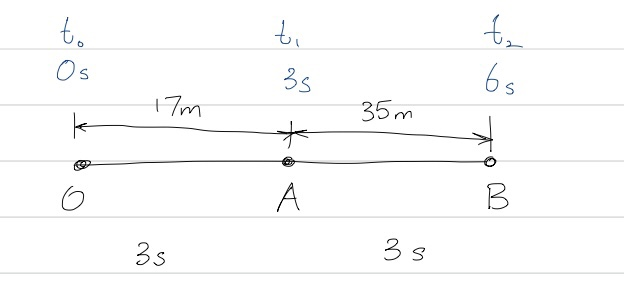
\includegraphics[scale=0.5]{../2010/figures/2010q5}
		\caption{\label{2010:q5:Move1} The relative positions of the particle while moving from $O$ to $B$.}
	\end{center}
\end{figure}
\rfig{2010:q5:Move1} shows the distances between the points that the particle moves to. As we want to find the acceleration of the particle, we should begin thinking about what we know (from the question) about the particle's motion and how we can use our knowledge of acceleration and motion in order to form a solution.





\textbf{\textit{Simplify and Diagram:}} \\ \\
\begin{figure}[H]
	\begin{center}
		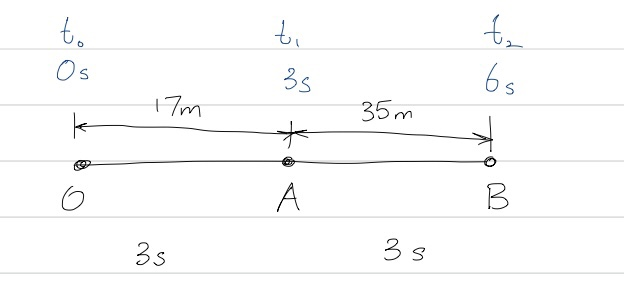
\includegraphics[scale=0.5]{../2010/figures/2010q5}
		\caption{\label{2010:q5:Move2} Diagram of the particle's motion, with relevant directions and distances.}
	\end{center}
\end{figure}
We are given that the particle takes 3 seconds cover $OA$ and $AB$. We are given time, distance, and a constant acceleration. Therefore, using our equations of motion (constant acceleration), we can formulate 2 equations and solve them simultaneously.
We will define:
\begin{itemize}
	\item $s$ is the displacement of the particle,
	\item $v$ is the final velocity of the particle,
	\item $u$ is the initial velocity of the particle,
	\item $a$ is the acceleration of the particle,
	\item $t$ is the time variable,
	\item $t(k)$ is the time taken to travel distance $k$.
\end{itemize}



\textbf{\textit{Represent Mathematically:}} \\ \\
Due to the quantities that we are given, we will use,
\begin{equation}
	s = ut + \frac{1}{2}at^2 \,.
\end{equation}




\textbf{\textit{Solve and Evaluate:}} \\ \\
Considering the distance $OA$, we get,
\begin{align}
	17 & = ut_1 + \frac{1}{2}at_1^2 \nn \\
	& = 3u + \frac{9}{2}a \,. \label{2010:q5:MoveEqn1}
\end{align}

We know that the distance $OB$ is the sum of the distances $OA$+$AB$. We also know that the time it takes for the particle to cover $OB$ is $t(OA)+t(AB)=6$. Therefore, we get that,
\begin{align}
	17+35 & = ut_2 + \frac{1}{2}at_2^2 \nn \\
	52 & = 6u + \frac{36}{2}a \,. \label{2010:q5:MoveEqn2}
\end{align}

We can solve \req{2010:q5:MoveEqn1} and \req{2010:q5:MoveEqn2} simultaneously by,
\begin{align}
	\text{(\req{2010:q5:MoveEqn2} - (2 $\times$ \req{2010:q5:MoveEqn1}))}:(52) - 2[17] & = \left(6u + \frac{36}{2}a\right) - 2\left[3u + \frac{9}{2}a\right] \nn \\
	                                                              52 - 34 & = \left(6u + 18a\right) - \left[6u + 9a\right] \nn \\
	                                                                   18 & = 9a \nn \\
	                                                                   \implies a & = 2\text{ms}^{-2} \,.
\end{align}

%------------------------------------------------------------------------------

\subsubquestion

\textbf{\textit{Simplify and Diagram:}} \\ \\
\begin{figure}[H]
	\begin{center}
		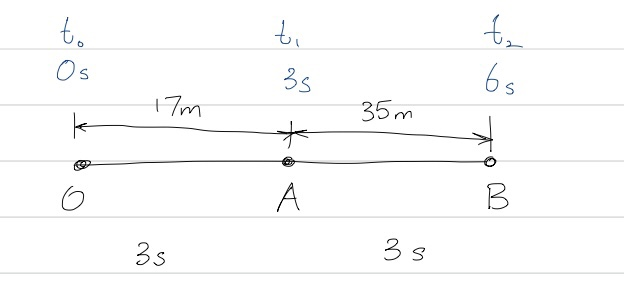
\includegraphics[scale=0.5]{../2010/figures/2010q5}
		\caption{\label{2010:q5:Move3} Diagram of the particle's motion, with relevant directions and distances.}
	\end{center}
\end{figure}
We want to find the time it takes for the particle to travel 105m away from $O$. We have values for the displacement and acceleration of the particle. This is not enough to solve for a time variable as we need at least 3 quantities to use our equations of motion. However, using the same sets of equations we derived in (5)(a)(i), we can find the value of the initial velocity $u$ and consequently solve for the time variable in the equation.




\textbf{\textit{Represent Mathematically:}} \\ \\
After we solve for $u$, we can use the equation,
\begin{equation}
	s=ut+\frac{1}{2}at^2 \,.
\end{equation}

Substituting our values, we will need to solve for $t$ in the equation,
\begin{align}
	105 & = ut+\frac{1}{2}(2)t^2 \nn \\
		\implies t^2 +ut -105 & = 0 \,.
\end{align}




\textbf{\textit{Solve and Evaluate:}} \\ \\
Firstly, using the value of $a$ that we found previously, we can substitute it into \req{2010:q5:MoveEqn2} and solve as,
\begin{align}
	52 & = 6u + \frac{36}{2}a \nn \\
	52 & = 6u + 18(2) \nn \\ 
	\frac{52-36}{6} & = u \nn \\
	\implies u & = \frac{8}{3}\text{ms}^{-1} \,.
\end{align}

Next, we can solve our quadratic in $t$ to obtain,
\begin{align}
	t^2 +ut -105 & = 0 \nn \\
	t^2 +\frac{8t}{3} -105 & = 0 \nn \\
	\implies t & = 9 ~\text{and}~\frac{-35}{3} \,.
\end{align}

Therefore, the time taken to travel 105m from $O$ is 9s.\footnote{We can make sense of the negative value by looking at the $s-t$ graph of the particle. We have arbitrarily labeled the $s=0$ point as $O$. If we consider the motion of the particle before $t=0$, we can see that there is a point where the distance of the body from $O$ was 105m. However, it was in the negative direction.}
\begin{figure}[H]
	\begin{center}
		\includegraphics[scale=1]{../2010/figures/2010q5-s-t-graph}
		\caption{\label{2010:q5:stGraph} Displacement time graph of the particle.}
	\end{center}
\end{figure}



\end{subsubquestions}
	
%------------------------------------------------------------------------------
% 5 b
%------------------------------------------------------------------------------
	
\subquestion

\begin{subsubquestions}
This part of the question uses the exact same reasoning from part (a), with different quantities to substitute and solve.

\subsubquestion
\textbf{\textit{Sketch and Translate:}} \\ \\
\begin{figure}[H]
	\begin{center}
		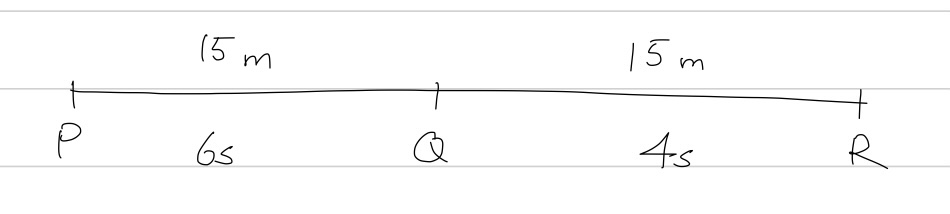
\includegraphics[scale=0.5]{../2010/figures/2010q5-2}
		\caption{\label{2010:q5:Move4} The relative positions of the particle while moving from $P$ to $R$.}
	\end{center}
\end{figure}
\rfig{2010:q5:Move4} shows the distances between the points that the particle moves to. As we want to find the acceleration of the particle, we should begin thinking about what we know (from the question) about the particle's motion and how we can use our knowledge of acceleration and motion in order to form a solution.





\textbf{\textit{Simplify and Diagram:}} \\ \\
\begin{figure}[H]
	\begin{center}
		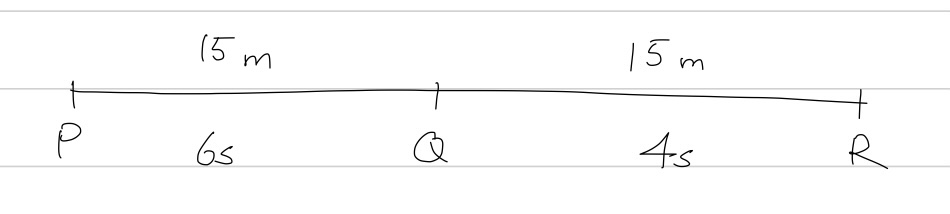
\includegraphics[scale=0.5]{../2010/figures/2010q5-2}
		\caption{\label{2010:q5:Move5} Diagram of the particle's motion, with relevant directions, distances and time.}
	\end{center}
\end{figure}
We are given that the particle takes 4s to cover $PQ$ and 6s to cover $QR$. We are given time, distance, and a constant acceleration. Therefore, using our equations of motion (constant acceleration), we can formulate 2 equations and solve them simultaneously.




\textbf{\textit{Represent Mathematically:}} \\ \\
Due to the quantities that we are given, we will use,
\begin{equation}
	s = ut + \frac{1}{2}at^2 \,.
\end{equation}




\textbf{\textit{Solve and Evaluate:}} \\ \\
Considering the distance $PQ$, we get,
\begin{align}
	15 & = ut_1 + \frac{1}{2}at_1^2 \nn \\
	& = 6u + \frac{36}{2}a \,. \label{2010:q5:MoveEqn3}
\end{align}

We know that the distance $PR$ is the sum of the distances $PQ$+$QR$. We also know that the time it takes for the particle to cover $PR$ is $t(PQ)+t(QR)=10$. Therefore, we get that,
\begin{align}
	15+15 & = ut_2 + \frac{1}{2}at_2^2 \nn \\
	30 & = 10u + \frac{100}{2}a \,. \label{2010:q5:MoveEqn4}
\end{align}

We can solve for the acceleration of the particle as follows,
\begin{align}
	(\text{3$\times$\req{2010:q5:MoveEqn4} - 5$\times$\req{2010:q5:MoveEqn3}}): (3 \times 30) - [5 \times 15] & = 3(10u+50a) - 5[6u+18a] \nn \\
                                                                                                    (90)-[75] & = (30u+150a)-[30u+90a] \nn \\
                                                                                                           15 & = 60a \nn \\
                                                                                                           \implies a & = \frac{1}{4}\text{ms}^{-2} \,.
\end{align}

%------------------------------------------------------------------------------

\subsubquestion
\textbf{\textit{Simplify and Diagram:}} \\ \\
\begin{figure}[H]
	\begin{center}
		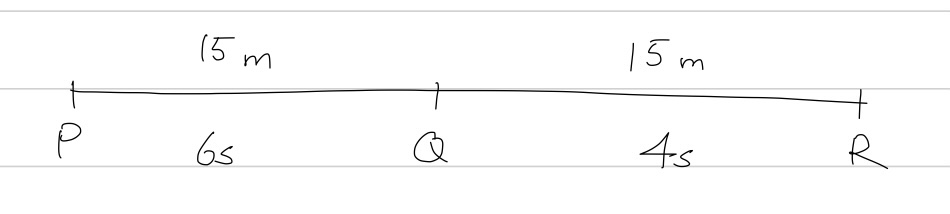
\includegraphics[scale=0.5]{../2010/figures/2010q5-2}
		\caption{\label{2010:q5:Move6} Diagram of the particle's motion, with relevant directions, distances and time.}
	\end{center}
\end{figure}
We want to find the velocity of the particle at a distance of 50m away from $P$. We have the acceleration and displacement from $P$, but this is not enough to motivate a solution. We can, however, obtain a value for the intial velocity, $u$, using the equations from part (b)(i). Therefore, using initial velocity, displacement, and acceleration, we can employ our equations of motion (constant acceleration) and find a value for the final velocity $v$.




\textbf{\textit{Represent Mathematically:}} \\ \\
After solving for $u$, we can use the equation,
\begin{align}
	v^2 & = u^2 + 2as \label{2010:q5:MoveEqn5} \,. 
\end{align}




\textbf{\textit{Solve and Evaluate:}} \\ \\
Firstly, using the value of $a$ that we found previously, we can substitute it into \req{2010:q5:MoveEqn4} and solve as,
\begin{align}
	30 & = 10u + \frac{100}{2}\left(\frac{1}{4}\right)a \nn \\
	   & = 10u + 50\left(\frac{1}{4}\right) \nn \\
	   \implies u & = \frac{30-12.5}{10} \nn \\
	   & = 1.75 \text{ms}^{-1} \,.
\end{align}

Substituting our values into \req{2010:q5:MoveEqn5}, we get that,
\begin{align}
	v^2 & = u^2 + 2as \nn \\
	\implies v & = \sqrt{u^2+2as} \nn \\
	  & = \sqrt{1.75^2+2(0.25)(50)} \nn \\
	  & = \sqrt{28.0625} \nn \\
	  & =  5.297 \text{ms}^{-1} \,.
\end{align}

\end{subsubquestions}
	
\end{subquestions}